\documentclass[a4paper]{article}
\usepackage[english]{babel}
\usepackage[english]{isodate}  		% english date format
\usepackage{textcomp, gensymb}      % to avoid some warnings
\usepackage{graphicx}				% image management
\usepackage{amsfonts}               % math fonts
\usepackage{booktabs}				% improve tables
\usepackage{amsmath}				% another math. pack.
% \usepackage{mathtools}				% underline under eq.
% \usepackage{stmaryrd} 				% for '\llbracket' and '\rrbracket'
% \usepackage{amsthm}					% better theorems
\usepackage{enumitem}				% list management
\usepackage{pifont}					% 'cute' bullet points
% \usepackage{cancel}					% cancel math expressions
\usepackage{caption}				% custom caption
\usepackage[]{mdframed}				% text box
\usepackage{multirow}				% table rows
\usepackage{gensymb}				% degree symbol
\usepackage[x11names]{xcolor}		% RGB colors pack.
\usepackage{tcolorbox}				% color box text

% draw a frame around given text
\newcommand{\framedtext}[1]{%
	\par%
	\noindent\fbox{%
		\parbox{\dimexpr\linewidth-2\fboxsep-2\fboxrule}{#1}%
	}%
}

% hypertext
\usepackage{xcolor}
\usepackage[linkcolor=black, citecolor=blue, urlcolor=cyan]{hyperref}
\hypersetup{
	colorlinks=true
}

% sorry, I don't use a US keyboard
\newcommand{\dquotes}[1]{``#1''}
\newcommand{\longline}{\noindent\rule{\textwidth}{0.4pt}}

\begin{document}
    \author{VR443470 - Valentini Andrea}
    \title{University of Verona \\
    \:\\
    AWS: EC2 F1 - Guide}
    \date{Last Update: \today}

    \maketitle

    \newpage

    \tableofcontents

    \newpage

    \section{Introduction to AWS}

    This guide was made to help some developers, and not, to understand how-to-use an AWS's product: EC2 F1. Note: obviously this is an unofficial guide.

    \longline
    
    \subsection{Register a new account}

    From this site you can register on the AWS platform: \url{https://aws.amazon.com/}. You can create an account choosing two possibility plans:
    \begin{itemize}
        \item Personal account, with some limitations (see more: \href{https://aws.amazon.com/free/?all-free-tier.sort-by=item.additionalFields.SortRank&all-free-tier.sort-order=asc&awsf.Free%20Tier%20Types=*all&awsf.Free%20Tier%20Categories=*all}{here});

        \item Business account, but attention because you need to register a payment card (see more: \href{https://aws.amazon.com/premiumsupport/plans/}{here}).
    \end{itemize}
    Although, there is an opportunity to students, and anyone else has an institutional e-mail, to register on the AWS Educate platform\footnote{FAQ: \url{https://www.awseducate.com/registration/s/faqs?language=en_US}}: \url{https://aws.amazon.com/education/awseducate/}. This plan allows you to access to AWS Educate lab, which provides access to the AWS Console to enable practical application of concepts without the need for credits (in summary, more resources without having to pay).\newline
    Unfortunately, Education Plan doesn’t give you the \dquotes{freedom} to do whatever you want because use AWS Console only meanwhile a learn course (sandbox).
    This choice is still valid because you can use the various tutorials to create guides (like this) or understand how-to-use EC2 F1.
    \begin{figure}[!htp]
        \centering
        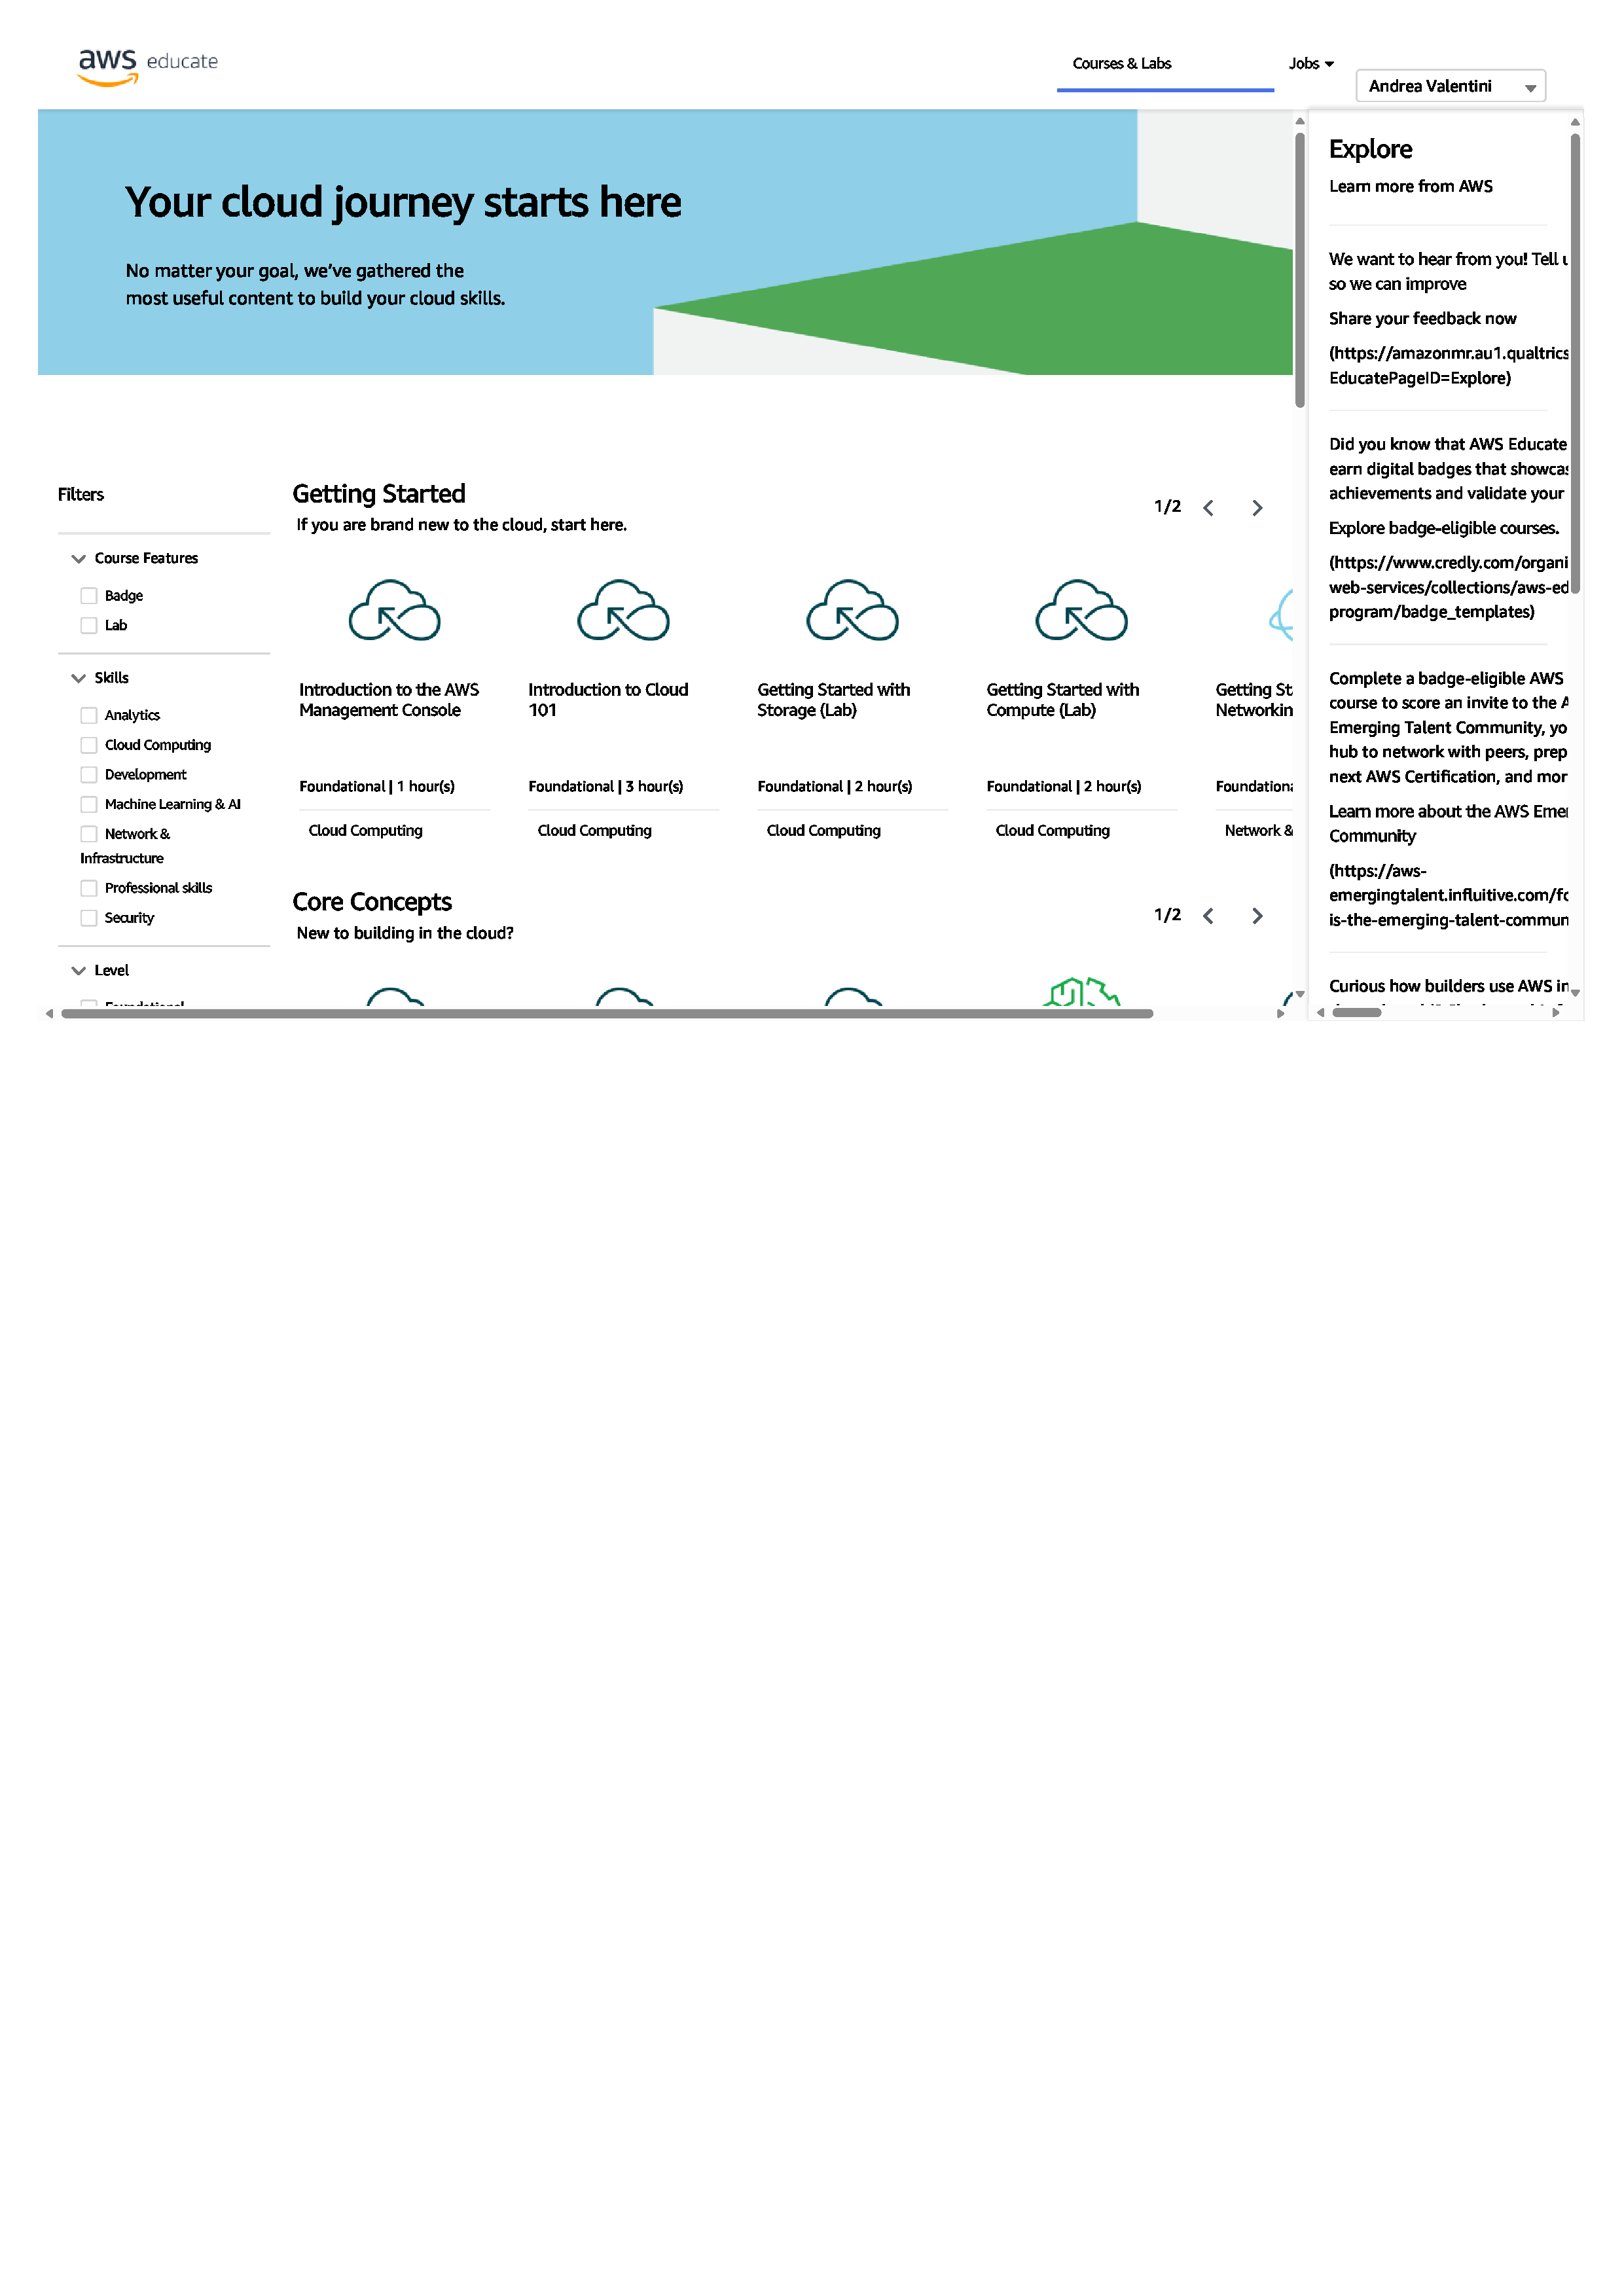
\includegraphics[width=\textwidth]{img/AWS Educate Dashboard.pdf}
        \caption{AWS Educate Dashboard.}
    \end{figure}\newpage

    \noindent
    If you've chosen to use a personal/business plan, once inserted a pay card number, and confirmed it with a 1\$ fee you should have this screen:
    \begin{figure}[!htp]
        \centering
        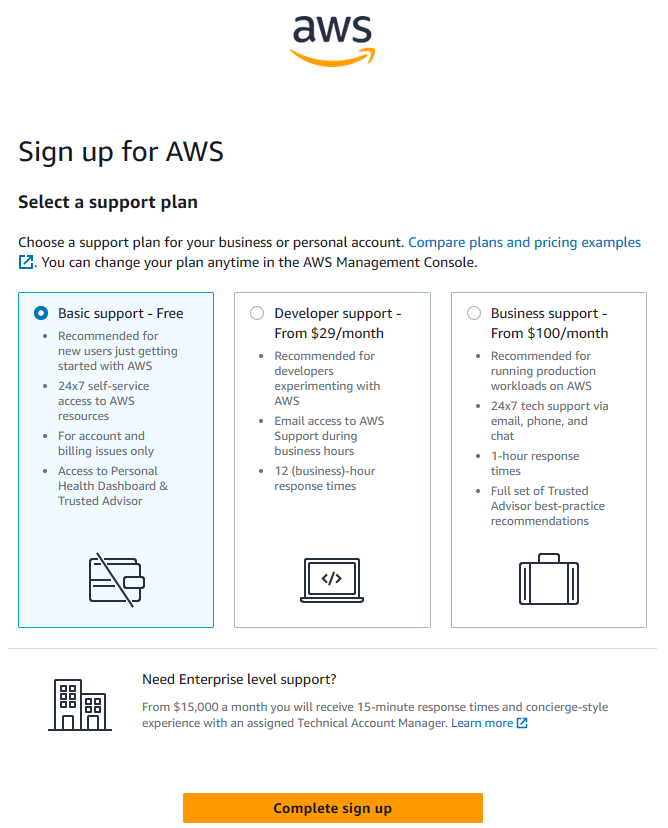
\includegraphics[width=\textwidth]{img/sing-up.png}
    \end{figure}

    \noindent
    On this figure, you can also see the various plans offered. To compare plans and pricing examples, you can visit this page: \href{https://aws.amazon.com/premiumsupport/plans/}{link}.\newline

    \noindent
    Anyway, choosing a Free plan will automatic start an AWS Free Tier (\href{https://aws.amazon.com/free/terms/}{terms}). The 12 Month Free Tier is only available to new AWS customers, and is available for 12 months following your AWS sign-up date.

    If you have not used the AWS resources provided under an Offer during the previous 3 months, we may reclaim those AWS resources after giving you 30 days’ notice. Even if your AWS resources are reclaimed, you may continue to participate in Offers using new AWS resources.

    \newpage

    \subsection{Getting Started}

    The first thing to do to understand how AWS works is read the Getting Started guide: \url{https://aws.amazon.com/getting-started/}. In this site, you can find some useful guides that explain cloud functions and others Amazon products.\newline

    \noindent
    After that, AWS shows you a sea of tutorials such as \dquotes{Build a Serverless Web Application}, \dquotes{Deploy a Web Application on Amazon EC2}, etc. Here's the link: \href{https://aws.amazon.com/getting-started/hands-on/?pg=gs&sec=lyfa&getting-started-all.sort-by=item.additionalFields.content-latest-publish-date&getting-started-all.sort-order=desc&awsf.getting-started-category=*all&awsf.getting-started-content-type=*all}{Hands-on Tutorials}.\newline

    \noindent
    If you chosen a Business (or free) account plan, this is your dashboard:
    \begin{figure}[!htp]
        \centering
        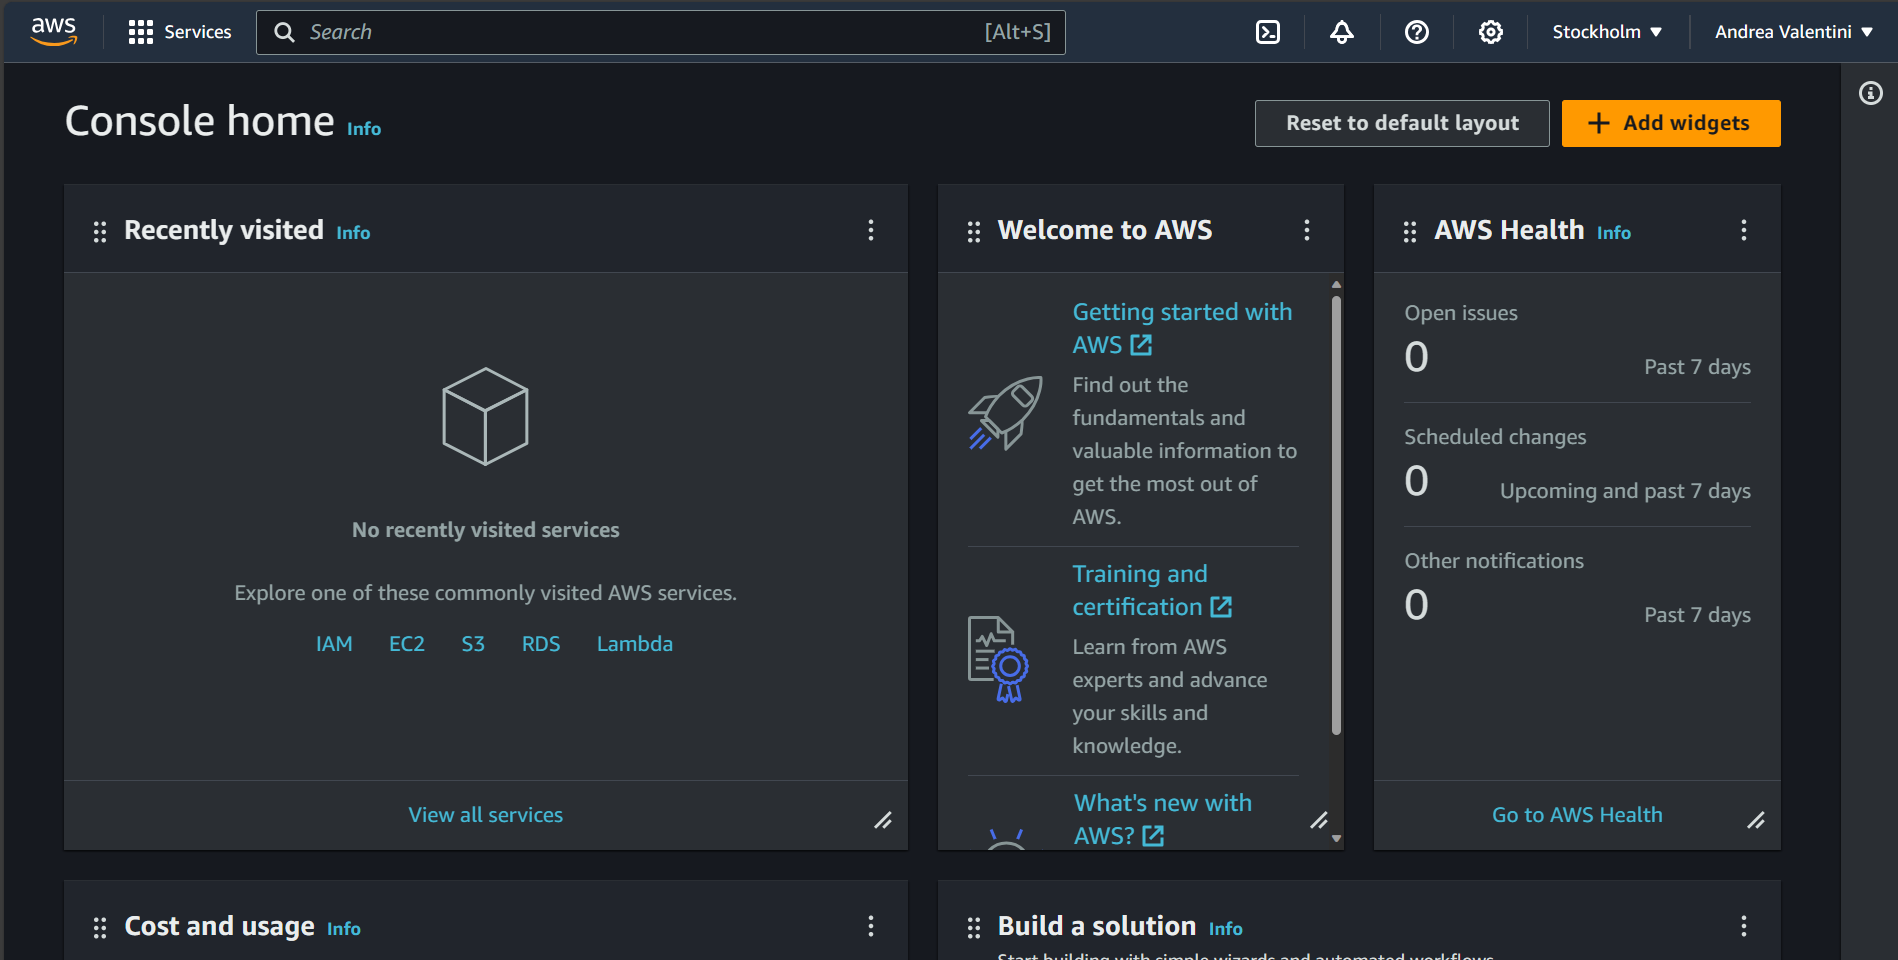
\includegraphics[width=\textwidth]{img/business-free_dashboard.png}
        \caption{AWS Business/Free Dashboard.}
    \end{figure}

    \noindent
    On the left side you can see all resources created and recently visited; at the top you can see all hypertext link that can help you to start.\newpage

    \section{Introduction to Amazon EC2 F1 Instances}

    \subsection{Description}

    Amazon EC2 F1 instances use FPGAs to enable delivery of custom hardware accelerations. With F1 instances you can:
    \begin{itemize}
        \item Develop
        \item Simulate
        \item Debug
        \item Compile
    \end{itemize}
    hardware acceleration code, including an FPGA Developer AMI (see \ref{sec: FPGA Developer AMI} cap.). Furthermore, EC2 supporting hardware level development on the cloud.\newline

    \noindent
    F1 instances provide diverse development environments: from low-level hardware developers to software developers who are more comfortable with C/C++ and openCL environments (see more on \ref{sec: development kit} par.).\newline

    \noindent
    Once your FPGA design is complete, you can register it as an Amazon FPGA Image (AFI), and deploy it to your F1 instance in just a few clicks. You can reuse your AFIs as many times as you like, and across as many F1 instances as you like. There is no software charge for the development tools when using the FPGA developer AMI and you can program the FPGAs on your F1 instance as many times as you like with no additional fees.\newline

    \noindent
    Instances Features:
    \begin{itemize}
        \item High frequency Intel Xeon Scalable Processors (Broadwell E5-2686 v4)
        \item NVMe SSD Storage
        \item Support for Enhanced Networking
    \end{itemize}
    FPGA Features:
    \begin{itemize}
        \item Xilinx Virtex UltraScale+ VU9P FPGAs
        \item 64 GiB of ECC-protected memory on 4x DDR4
        \item Dedicated PCI-Express x16 interface
        \item Approximately 2.5 million logic elements
        \item Approximately 6,800 Digital Signal Processing (DSP) engines
        \item FPGA Developer AMI (see \ref{sec: FPGA Developer AMI})
    \end{itemize}\newpage

    \begin{table}[!htp]
        \centering
        \begin{tabular}{@{} l p{4em} p{4em} p{4em} p{4em} p{6em} @{}}
            \toprule
            \textbf{Instance} & \textbf{FPGAs} & \textbf{vCPU} & \textbf{Memory (GiB)} & \textbf{Instance Storage (GB)} & \textbf{Networking Performance (Gbps)***} \\
            \midrule
            \texttt{f1.2xlarge}     & 1 & 8 & 122 & $1 \times 470$ & Up to 10 \\
            \texttt{f1.4xlarge}     & 2 & 16 & 244 & $1 \times 940$ & Up to 10 \\
            \texttt{f1.16xlarge}    & 8 & 64 & 976 & $4 \times 940$ & 25 \\
            \bottomrule
        \end{tabular}
    \end{table}
    For \texttt{f1.16xlarge} instances, the dedicated PCI-e fabric lets the FPGAs share the same memory space and communicate with each other across the fabric at up to 12 Gbps in each direction.\newline

    \noindent
    All instances have the following specs:
    \begin{itemize}
        \item 2.3 GHz (base) and 2.7 GHz (turbo) Intel Xeon E5-2686 v4 Processor

        \item \href{https://aws.amazon.com/ec2/instance-types/#Intel}{Intel AVX*, Intel AVX2*, Intel Turbo}

        \item \href{https://aws.amazon.com/ec2/instance-types/#EBS}{EBS Optimized}

        \item \href{https://aws.amazon.com/ec2/details/#enhanced-networking}{Enhanced Networking*}
    \end{itemize}
    * AVX and AVX2 are only available on instances launched with HVM AMIs.\newline

    \noindent
    *** Instances marked with "Up to" Network Bandwidth have a baseline bandwidth and can use a network I/O credit mechanism to burst beyond their baseline bandwidth on a best effort basis. For more information, see \href{https://docs.aws.amazon.com/AWSEC2/latest/UserGuide/ec2-instance-network-bandwidth.html}{instance network bandwidth}.

    \longline

    \subsection{Development Kit}\label{sec: development kit}

    Once you created an AWS account, you \textbf{must} downloading the AWS FPGA Development Kit by this official repository: \url{https://github.com/aws/aws-fpga}. It includes all documentation (\href{https://github.com/aws/aws-fpga#documentation-overview}{shortcut url}) on:
    \begin{itemize}
        \item F1
        \item Internal FPGA interfaces
        \item Compiler scripts for generating Amazon FPGA Images (AFIs)
    \end{itemize}
    
    \noindent
    AWS FPGAs support multiple development environments to serve both hardware and software developers:
    \begin{itemize}
        \item The FPGA Hardware Development Kit (HDK, \href{https://github.com/aws/aws-fpga#hardware-development-kit-hdk}{shortcut url}) provides fully custom hardware development;

        \item The FPGA Software Development Kit (SDK, \href{https://github.com/aws/aws-fpga#runtime-tools-sdk}{shortcut url}) environment allows developing accelerations using C/C++/OpenCL code with no hardware knowledge needed.
    \end{itemize}
    Again, this kit is \textbf{essential to develop fast FPGA for the EC2 F1 instances}.\newpage

    \subsection{FPGA Developer AMI}\label{sec: FPGA Developer AMI}

    The FPGA Developer AMI is an Amazon Linux 2 based AMI provided by Amazon Web Services. The AMI is pre-built with FPGA development tools required to develop and use custom FPGAs for hardware acceleration. The FPGA Developer AMI includes Xilinx tools for simulating your FPGA design, compiling code and building your AFI (Amazon FPGA Image).\newline

    \noindent
    The FPGA Developer AMI includes Xilinx Vivado\footnote{Xilinx Vivado is a software suite produced by AMD (previously Xilinx) for synthesis and analysis of hardware description language (HDL) designs, superseding Xilinx ISE with additional features for system on a chip development and high-level synthesis. \href{https://en.wikipedia.org/wiki/Vivado}{Source}.} at no additional software charge as well as a prepackaged tool development environment with scripts and tools for simulating your FPGA design and building and registering your AFI.\newline

    \noindent
    As mentioned above, developers can deploy the FPGA Developer AMI on an Amazon EC2 instance and quickly provision the resources they need to write and debug FPGA designs in the cloud. The FPGA Developer AMI is provided at no additional charge to Amazon EC2 users.\newline

    

    \noindent
    Typical Total Price (updated on 17th October 2023): \$0.796/hr.\newline

    \noindent
    See more: \href{https://aws.amazon.com/marketplace/pp/prodview-iehshpgi7hcjg}{AWS marketplace}\newpage

    \subsection{Some interesting blog posts \& articles}

    \begin{itemize}
        \item \href{https://aws.amazon.com/blogs/publicsector/university-of-berkeley-uses-aws-educate-for-amazon-fpga-accelerator-development-and-deployment-in-the-cloud/}{University of California, Berkeley uses AWS Educate and Amazon FPGA Instances in Undergraduate Computer Architecture Course} by AWS Public Sector Blog Team

        \item \href{https://aws.amazon.com/blogs/startups/competition-forever-change-blockchain/}{Time, Randomness, and a \$100,000 Prize to Forever Change Blockchain} by Michael V. Copeland

        \item \href{https://aws.amazon.com/blogs/apn/how-dnanexus-and-edico-genome-are-powering-precision-medicine-on-amazon-web-services-aws/}{How DNAnexus and Edico Genome are Powering Precision Medicine on Amazon Web Services (AWS)} by Aaron Friedman and Ujjwal Ratan

        \item \href{https://aws.amazon.com/blogs/compute/bringing-datacenter-scale-hardware-software-co-design-to-the-cloud-with-firesim-and-amazon-ec2-f1-instances/}{Bringing Datacenter-Scale Hardware-Software Co-design to the Cloud with FireSim and Amazon EC2 F1 Instances} by Mia Champion

        \item \href{https://aws.amazon.com/blogs/compute/accelerating-precision-medicine-at-scale/}{Accelerating Precision Medicine at Scale} by Aaron Friedman and Angel Pizarro
    \end{itemize}\newpage

    \section{AWS EC2 FPGA Development Kit}
\end{document}